Как было выяснено, при наблюдении далёких предметов с помощью астрономической
зрительной трубы (трубы Кеплера) глазом, аккомодированным на бесконечность, задний фокус 
объектива совпадает с передним фокусом окуляра. В этом случае труба является \textit{афокальной 
системой}: параллельный пучок лучей, входящий в объектив, остаётся параллельным по выходе
из окуляра. Такой ход лучей называют \textit{телескопическим}.

\begin{figure}[h]
  \center{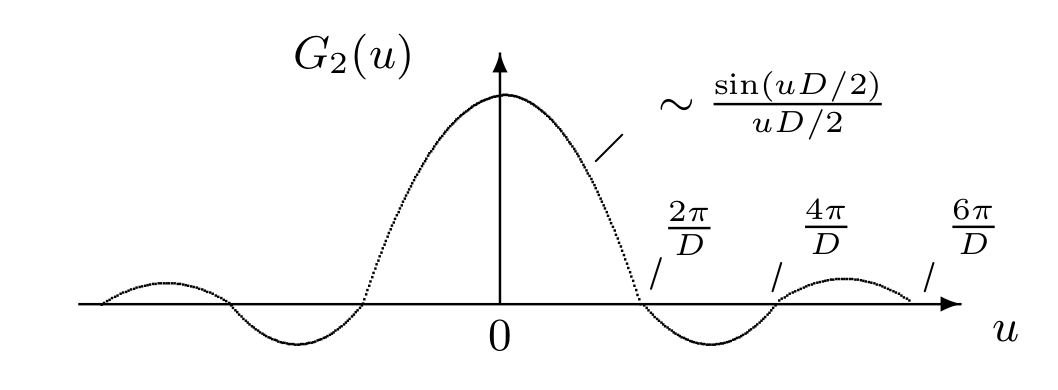
\includegraphics[width=\linewidth]{4.png}}
  \caption{К расчёту увеличения зрительной трубы Кеплера}
  \label{img::4}
\end{figure}

Рассматривая параллельный пучок лучей, исходящий из бесконечно удалённой точки, лежащей 
в стороне от оптической оси, можно для простоты ограничиться лучом, проходящим через 
центр объектива (рис. \ref{img::4}а). На выходе из окуляра угол наклона пучка к оптической 
оси изменяется.

Пусть пучок света, попадающий в объектив, составляет с оптической осью угол $\varphi_1$, 
а пучок, выходящий из окуляра, -- угол $\varphi_2$. Увеличение $\gamma$ зрительной трубы по 
определению равно

\begin{equation}\label{eq::1}
  \gamma = \frac{\tg \varphi_2}{\tg \varphi_1}
\end{equation}

Строго говоря, $\varphi_1$ -- это угловой размер объекта, рассматриваемого невооружённым 
глазом, но при наблюдении бесконечно удалённого объекта с помощью зрительной трубы угол
$\varphi_1$ для объектива трубы и для невооружённого глаза одинаков. Как следует из 
рис. \ref{img::4}а, угловое увеличение телескопа равно отношению фокусов объектива и окуляра:

\begin{equation}\label{eq::2}
  \gamma = \frac{\tg \varphi_2}{\tg \varphi_1} = \frac{f_1}{f_2}
\end{equation}

Отношение фокусных расстояний равно отношению диаметров пучка, прошедшего объектив и 
окуляр (рис. \ref{img::4}б). Ширина пучка, прошедшего объектив, определяется диаметром $D_1$ 
его оправы; ширина пучка, выходящего из окуляра, -- диаметром $D_2$ изображения оправы
объектива, даваемого окуляром:

\begin{equation}\label{eq::3}
  \frac{f_1}{f_2} = \frac{D_1}{D_2}
\end{equation}

Таким образом, угловое увеличение телескопа

\begin{equation}\label{eq::4}
  \gamma = \frac{\tg \varphi_2}{\tg \varphi_1} = \frac{f_1}{f_2}  = \frac{D_1}{D_2}
\end{equation}

В том случае, когда диаметр $D_2$ пучка, выходящего из окуляра, равен диаметру $d_0$ 
зрачка наблюдателя ($d_0 \approx 5$ мм), увеличение телескопа называется нормальным.
Соотношение \eqref{eq::4} показывает, что увеличение трубы можно определить следующими 
тремя способами: путём измерения углов, под которыми предмет виден через трубу и без неё, 
путём измерения диаметров объектива и его изображения в окуляре, и наконец, путём 
измерения фокусных расстояний объектива и окуляра. В настоящей работе используются
все три способа.
